\subsection{Arc length}

Let $g(t)$ be a function that draws a curve.
The arc length from $g(a)$ to $g(b)$ is given by
$$\int_a^b|g'(t)|\,dt$$
For example, let us measure the length of

\medskip
\verb$xrange=(0,1)$

\verb$yrange=(0,1)$

\verb$draw(x^2)$

\begin{center}
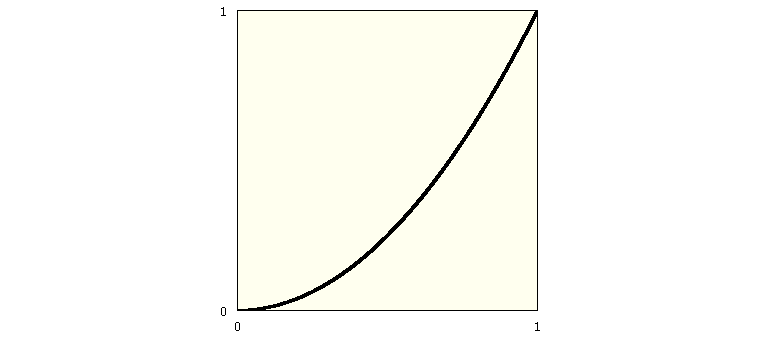
\includegraphics[scale=0.4]{arc.png}
\end{center}

\medskip
\noindent
A suitable $g(t)$ for the arc is
$$g(t)=\left(\matrix{t\cr t^2}\right),\quad0\le t\le1$$
The Eigenmath solution is

\medskip
\verb$g=(t,t^2)$

\verb$defint(abs(d(g,t)),t,0,1)$

$$\hbox{$1\over4$}\log(2+5^{1/2})+\hbox{$1\over2$}5^{1/2}$$

\verb$float$

$$1.47894$$

\medskip
\noindent
As we would expect, the result is greater than $\sqrt2$, the length of the
diagonal.

\medskip
\noindent
The result seems rather complicated given that we
started with a simple parabola.
Let us inspect $|g'(t)|$ to see why.

\medskip
\verb$g$

$$g=\left(\matrix{t\cr t^2}\right)$$

\medskip
\verb$d(g,t)$

$$\left(\matrix{1\cr2t}\right)$$

\medskip
\verb$abs(d(g,t))$

$$(4t^2+1)^{1/2}$$

\subsection{Line integrals}

Line integrals are easily computed by
converting the coordinates $x$, $y$ and $z$ into functions of $t$.
This has the effect of changing the measure as well.
For instance, $dx$ becomes $(dx/dt)\,dt$.
The following line integral problems are from
{\it Advanced Calculus, Fifth Edition} by Wilfred Kaplan.

\medskip
\noindent
Evaluate $\int y^2\,dx$ along the straight
line from $(0,0)$ to $(2,2)$.

\medskip
\verb$x=2t$

\verb$y=2t$

\verb$defint(y^2*d(x,t),t,0,1)$

$$8\over3$$

\medskip
\noindent
Evaluate $\int y\,dx$ along the straight line from
$(2,1)$ to $(1,2)$.

\medskip
\verb$x=2-t$

\verb$y=t+1$

\verb$defint(y*d(x),t,0,1)$

$$-{3\over2}$$

\medskip
\noindent
Evaluate $\int x\,dy$ along the straight line from
$(1,1)$ to $(2,1)$.

\medskip
\verb$x=t+1$

\verb$y=1$

\verb$defint(x*d(y),t,0,1)$

$$0$$

\medskip
\noindent
Evaluate $\int z\,dx+x\,dy+y\,dz$
along the path
$x=2t+1$, $y=t^2$, $z=1+t^3$, $0\le t\le 1$.

\medskip
\verb$x=2t+1$

\verb$y=t^2$

\verb$z=1+t^3$

\verb$f=z*d(x)+x*d(y)+y*d(z)$

\verb$defint(f,t,0,1)$

$$163\over30$$

